%--------------------------------------------%
% Packages arranged by : Tsz Timmy Chan	     %
%                 Date : November 26th, 2016%
%--------------------------------------------%

\documentclass{TC}
\usepackage{TCcommon}

\title{TITLE HERE}	% Work Title Here.
\author{Tsz Timmy Chan}	% YOUR NAME HERE 

\usepackage[notes]{TCheader}
\usepackage{TCexamtitle}
%\renewcommand{\benediction}{" " - }
%\renewcommand{\quoteoftheday}{" " \\ - }
\begin{document}


Since we currently do not have a theoretical approach to the cone conjecture aside from a direct proof in dimension 3, we used a computational approach for dimension 4 and 5 in the hopes for further insight. Below we present the details on the implementation of the two elementary extensions in higher dimensions. 


\section{Experimental Method} 
The exhaustive study of cones by computational means is challenging, even with severe restrictions on the number of extremal generators in $\Z^d$ to be some number close to $d$. Since we are studying full dimensional cones, all cones $C$ must have $\#\mathrm{Ext}(C) \geq d$, with further restrictions on the coordinates, the problem quickly becomes intractable. 

While we were not able to attempt an exhaustive search, the combinatorics question itself is interesting:

\noindent \textbf{Question.} How many full dimensional cones can we form in $\Z^d$ with $n \geq d$ vectors, where each extremal generator is in $\{\mathbf{x} \in \Z^d : 0\leq x_i \leq k\}$? 

Some work towards this: We have an upper bound, since this region has $(k+1)^d-1$ points, we have at most ${(k+1)^d-1 \choose n}$ choices, with an \emph{unknown} probability for the choices that are linearly independent. 

For our purposes, we would not only need the number of full dimensional cones, but also list these vectors explicitly; thus, we arranged the vectors as columns of a matrix, and attempt to find its determinate to check for linear independence. However, physically running this na\"ive algorithm will lead to astronomical numbers of steps, even for $d = 5$, $n = 5$ and $k = 2$, we would have to check $\displaystyle { 3^5 \choose 5} = {242 \choose 5} \approx 6.63 \times 10^{9} $ matrices. After collecting the linearly independent combinations, one must then find combinations that satisfy containment, and after that we decided that this path is physically impossible to do within the time constraints for a master's thesis. 

Thus, we utilize randomly generated pairs of full dimensional cones in order to examine the poset of cones. While most of our experiments use random cones, we have also included a simple text UI that allows for proper input of a list of extremal generators for a pair of cones, and the associated logical verification to ensure we satisfy the conditions associated with the cone conjecture.  

Furthermore, we give a full description of the two algorithms described below, and test whether the algorithms terminate. If the implementation show evidence that there are no non-terminating processes of either type, then this also gives strong evidence that the conjecture is true. Whenever the algorithms terminate, they give a finite sequence of cones from $C$ to $D$ that satisfy stricter conditions than the order statement.


\subsection{Technical Requirements}
The implementation of the experiment uses the development branch of \texttt{SAGE} \cite{sagemath}, and the PyNormaliz package to link \texttt{Normaliz} \cite{Normaliz}. The experiment was written in the standard python format. Finally, the experiment was run on the operating system \texttt{Ubuntu~16.04~LTS}. 

A current version of the code for this experiment is hosted on \texttt{GitHub} \cite{ChanGitHubMA}.

\section{Algorithms and Procedures}

\subsection{Terminal User Interface vs. Python Scripts}
As the way this experiment is designed, one may run experiments in batch by writing a script in Python, or use the built in terminal user interface. While simple, this terminal user interface was built from scratch using dictionaries and UI functions built over time. 

Using \texttt{JSON} file formats, the code is written so that a user may create a new experiment or load an incomplete experiment, and an option to copy an experiment either its current state or just the initial conditions.

In the creation of a new experiment, a user must first choose the dimension, and then set boundaries for the generation of cones or manually input vectors. The manual input part also does a simple sanity check, where it verifies:
\begin{enumerate}
\item Vectors are of the form $(x_1,...,x_d): x_i \in \Z \text{ for } i = 1,...,d$; 
\item The outer cone is full dimensional and pointed;
\item Each vector of the inner cone must be contained by the outer cone;
\item The inner cone must be full dimensional (if the outer cone is pointed then the inner cone is automatically pointed).
\end{enumerate}

\subsection{Randomly Generating Cones}
First, we generate random vectors, by using the built-in  \texttt{SAGE} random integer generators. In particular, we generate vectors in $\Z^d$ of the form $\{x_1 , \ldots, x_d\}$ where $ |x_i| \leq k$ for some sensible $k$ and $x_d > 0$, which forces our cones to be within one halfspace. In doing so, we do not lose generality, as by a simple affine transformation we can then study cones that are limited by other halfspaces.



For any experiment, the first step (if not by user input) is to initiate our data structures by randomly generating $C, D \in \Cones(d)$ where $C \subset D$ and satisfy the above conditions.
 
\begin{enumerate}
\item Retrieve a particular dimension $d$, and the user provides number of $n$ generators, either by a terminal user interface or by a constructor in a separate python script.

\item Unless the user specifies the cones, we generate vectors $\mathbf c_i \in \Z^d, i = 1, \ldots, n$, with a user chosen $n$ such that $n \geq d$ (so that we have a full-dimensional cone). We force each of the vectors $\mathbf c \in \{ x \in \Z^d : x_d > 0\}$.

\item We then take the conical hull of these randomly generated vectors, and then define this as our outer cone $D = \mathrm{Cone}(\{c_1,\ldots, c_n\})$, and repeat until the cone is full dimensional and we have $n$ rays. (Since some vectors may be linearly dependent, as $n$ grows large above $d$ this process of "organically" generating a cone may slow down.)

\item Next, we generate vectors randomly and check that each is contained in the outer cone $D$. Once we have $n$ vectors of this form, we take the conical hull. Using \texttt{SAGE}, we verify the cone must be full dimensional first. 

\end{enumerate}
These steps ensure that $C$ and $D$ are both pointed cones, with $C \subset D$. 






\subsection{Top Down}
\begin{figure}[h]
\centering
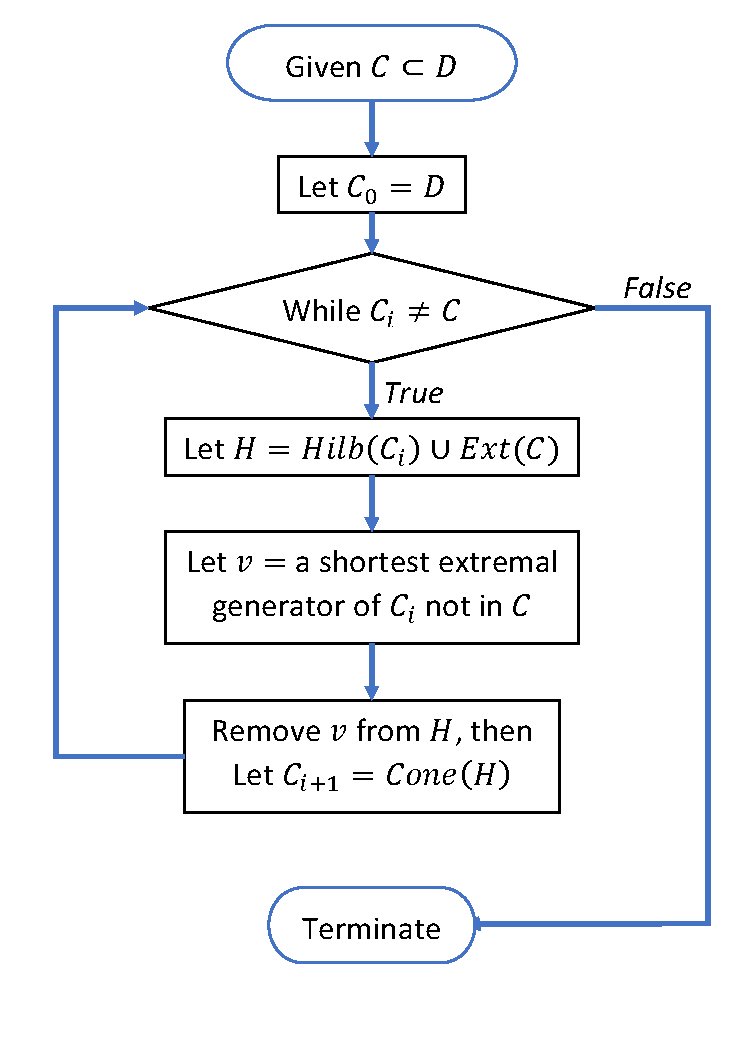
\includegraphics[width=.49\textwidth]{TopDownFC.pdf}
\caption{Flow chart for the \emph{Top Down} algorithm.}
\end{figure}
This algorithm uses Hilbert Descents to "shave" $D$ down to $C$.


\begin{enumerate}
\item Let $D_0 = D$, i.e., we set the initial cone to be the outer cone $D$.
\item Let $H = \mathrm{Hilb}(D_0)$, i.e., we collect the indecomposable elements of $L(D_0)$.
\item Let $D_1 = \mathrm{Cone}(H \takeaway \{v\})$, i.e., we take the conical hull of all the indecomposable elements of $L(D_0)$ after removing $v$ from the list.


\item While $D_i \neq C$, 
	\begin{enumerate}
	
		\item Let $H$ be a list containing the Hilbert basis of $D_{i}$. 
		\item Collect the set extremal generators of $D$ that are not in $C$ and collect these vectors into a list $E_{i} = \mathrm{ExtGen}(D_i) \cap C^c$.
		\item Loop through $E_{i}$ and record the lengths of each vector. Then choose one of the vectors with the smallest Euclidean norm from this list, call this $v_i$.
		\item Return $D_{i+1} = \mathrm{Cone}(\mathrm{Hilb}(D_i)\takeaway\{v_i\} \cup C)$, i.e., remove $v_i$ from the list $H$, and return the conical hull of $H \takeaway \{v_i\}$.
		
	\end{enumerate} 
\end{enumerate}


\subsection{Bottom Up}
We grow the inner cone to the outer cone by height-1 extensions. Previous results have shown that this method produces a cone more quickly than the \emph{Top Down} algorithm.

In order to describe the algorithm, we define a special type of polyhedron called a \emph{zonotope}:
\begin{definition}[Zonotope]
A zonotope is a set of points in $d$-dimensional space constructed from vectors $v_i$ by taking the sum of $a_iv_i$, where each  $a_i$ is a scalar between 0 and 1. Given $V = \{ v_1,\ldots, v_k\}$:
$$\mathrm{Zonotope(V)} = \{ x \in \R^d: x = a_1v_1 + \cdots + a_k v_k \text{ and } 0 \leq a_i \leq 1 \text{ for each } a_i \}.$$
\end{definition}
\begin{figure}[h]
\centering
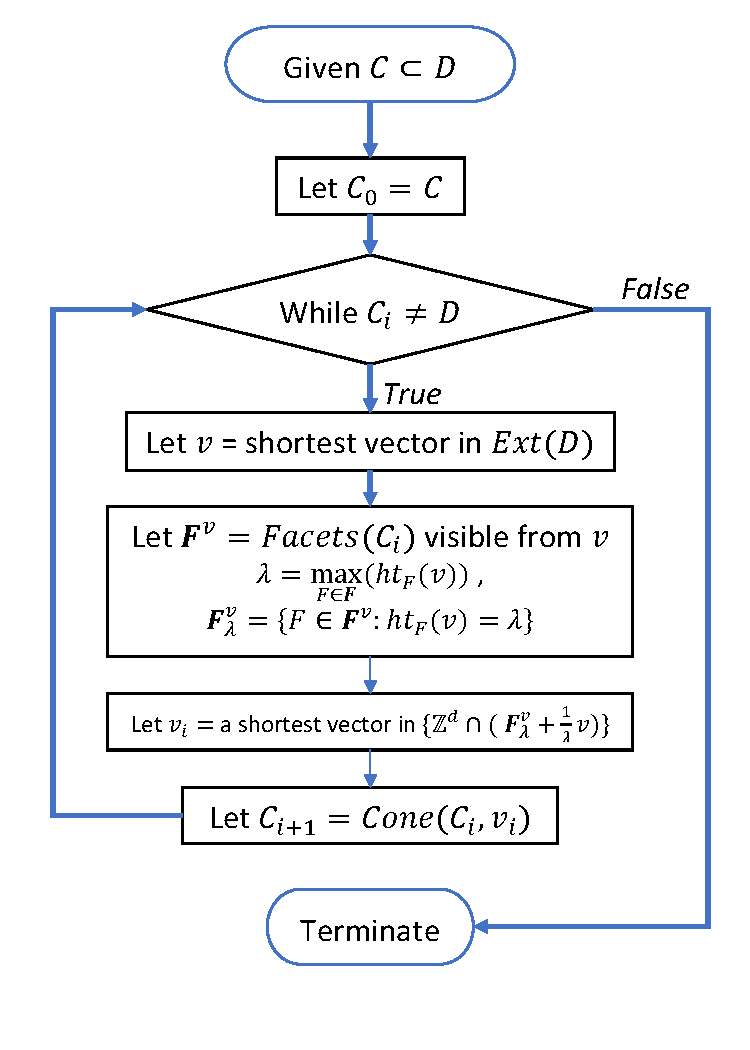
\includegraphics[width=.49\textwidth]{BottomUpFC.pdf}
\caption{Flow chart for the \emph{Bottom Up} algorithm.}
\end{figure}



\begin{enumerate}

\item Let $C_0 = C$.
\item While $C_i \neq D$:

\begin{enumerate}
\item Collect the set of facets of $C_i$  visible from $v$:
\begin{enumerate}
\item Let $\mathbb F^v$ be the set of facets of $C$ visible from $v$, i.e., $H_{\alpha}$ is a support hyperplane of $C$ associated with a facet $F$.
\item  $F$ is visible from $v$ if $C \subset H_{\alpha}^+ \implies v \subset (H_{\alpha}^+)^c$. Computationally, we can simply check that $C$ and $v$ have opposite signs when evaluated using $\alpha$; i.e., if $\alpha(c) < 0 $ for every $c \in C$, then $F$ is visible from $v$ if $\alpha(v) > 0$.
 
\end{enumerate}
\item Let $ht_{F}(v) = \alpha(v)$ given that $\alpha$ is the linear form associated with the support hyperplane of the facet $F$.
\item Let $\lambda = \displaystyle\max_{F \in \F}(ht_{F}(v))$. Collect the set $\F^v_\lambda = \{F \in \F^v: ht_{F}(v) = \lambda\}$. 
\item Shift this set $\F^v_{\lambda}$ along $\frac{1}{\lambda} v$, and find the shortest integer lattice point. Looping through each shifted facet $F$ in $\F^v_{\lambda}$:
	\begin{itemize}
	\item Computationally, we take the extremal generators of each facet $F$ and from a zonotope $Z_F$. Shift $Z_F$ by $\frac{1}{\lambda}v$.
	\item Once we have $Z_F + \frac{1}{\lambda}v$, collect the vectors $L(Z_F+\frac{1}{\lambda}v )$ and append this to a list $E_i$. 
\begin{remark}\label{zonotopelattice}
The zonotope $Z_F + \frac{1}{\lambda}v$ always contains at least one lattice element.
\end{remark}
	\end{itemize}
\item Loop through $E_i$ and find the shortest vector, called this $v_i$.
\item Return $C_{i+1} = \mathrm{Cone}(C \cup v_i)$. 
\end{enumerate}
\end{enumerate}





The two algorithms can be used alternatively, and we examine the difference of the two algorithms by comparing the number of elements of the Hilbert basis of each successive cone. 


\begin{lemma}
The \emph{Top Down} and \emph{Bottom Up} algorithms yield the same chain of cones in $\R^2$.
\end{lemma} 


\begin{figure}[h]
\begin{multicols}{2}
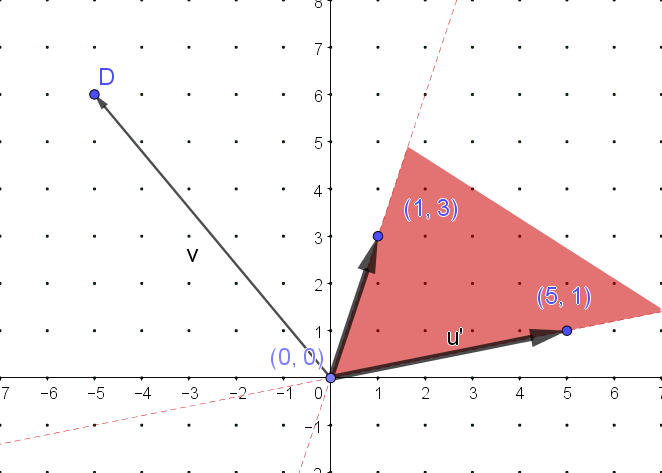
\includegraphics[width=.49\textwidth]{SimpleCone}
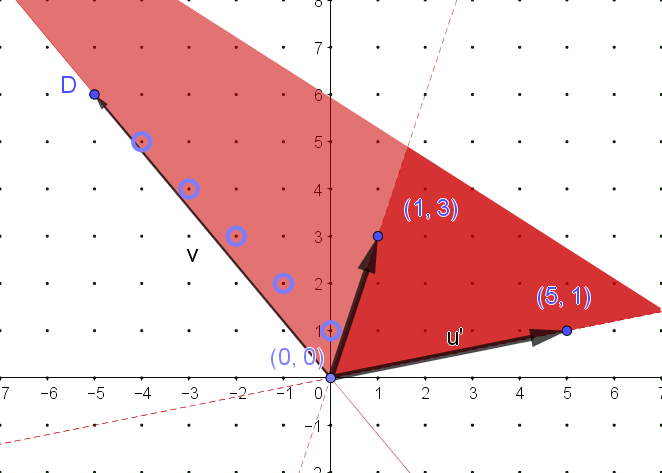
\includegraphics[width=.49\textwidth]
{SimpleCone2}
\end{multicols}

\caption{Demonstration of the \emph{Top Down} and \emph{Bottom Up} algorithms in $\R^2$.}
\end{figure}

Yet, for $d > 2$, in $\R^d$ the algorithms do not always generate the same cones, demonstrated in the data section below.




\section{Objects and Data Structure Overview}

\begin{figure}[h]
\centering
\includegraphics[width=.75\textwidth]{"Data Structure Picture"}
\caption{Visualization of Object-Oriented Design.}
\end{figure}
The object oriented version currently existing on \texttt{Github} allows for advantages over the procedural version in several ways. In particular, the Hilbert basis calculation for each cone used in the Top Down algorithm is computationally expensive, and the most elementary data structure in this design was created specifically to avoid doing multiple calculations on the same cone. 

Three central objects were created for this experiment, and here we present the essential attributes and methods of the code. The reader may find the source code in \textbf{Chapter~\ref{Source}}.

\begin{enumerate}
	
\item \texttt{cone\_chain\_element.py} Object file that contains a \texttt{SAGE} polyhedron object (which is our cone) and the associated data and methods:
	\begin{itemize}
	\item Essential Attributes:
		\begin{itemize}
		\item \texttt{cone, cone\_rays\_list}: The \texttt{SAGE} polyhedron object and the extremal generators of the cone.			
		\item \texttt{generation\_step, algorithm\_used}: to denote what step this cone was generated and what algorithm was used. 0 if initial cones. For algorithm used, the letter "i" denotes initial cone, "t" denotes top down, "b" denotes bottom up.
		\item \texttt{hilbert\_basis} Storing Hilbert basis of the cone in this object. This ensures that the calculation is only done once.
		\end{itemize}
	\item Essential Methods:
		\begin{itemize}
		\item \texttt{get\_hilbert\_basis(self)} Method to interface with the data in the object, with the logic to guarantee that \texttt{Normaliz} is used at most once for each \texttt{ConeChainElement} object.
		\item \texttt{output\_details(self)} Prints to terminal details about this particular cone. Used in other I/O methods elsewhere.
		\end{itemize}
	\end{itemize}
	
\item \texttt{cone\_chain.py} Object file that contains three lists of \texttt{ConeChainElements} designed to represent three valid cone poset chains. 
	\begin{itemize}
	\item Attributes:
		\begin{itemize}
		\item \texttt{inner\_cone, outer\_cone} the cones initializing the experiment.
		\item \texttt{top\_sequence}: first contains \texttt{outer\_cone}, then every cone generated by the \texttt{top\_down} algorithm.
		\item \texttt{bottom\_sequence}: first contains \texttt{inner\_cone}, then every cone generated by the \texttt{bottom\_up} algorithm.
		\item \texttt{cone\_chain}: generated only when the either \texttt{top\_down / bottom\_up} terminates, and arranges it so that the \texttt{inner\_cone} is the first element and the \texttt{outer\_cone} is the last element.
		\end{itemize}
	\item Methods:
		\begin{itemize}
		\item \texttt{top\_down} algorithm, implements Hilbert descends.
		\item \texttt{bottom\_up} algorithm, implements height-1 extensions.
		\end{itemize}
	\end{itemize}
\item \text{cone\_conjecture\_tester.py} Wrapper object that deals with all UI, creation/initialization of experiments, loading/saving operations. This also contains functions to generate graphs and save summaries.
\end{enumerate}


\end{document}